
\documentclass[10pt]{beamer}
\usepackage{amsmath}
\usepackage{mathtools}
\usepackage{multimedia}
\usepackage{hyperref}


\usefonttheme{professionalfonts} % using non standard fonts for beamer
\usefonttheme{serif} % default family is serif
%\documentclass[12pt]{beamerthemeSam.sty}
\usepackage{epsf}
%\usepackage{pstricks}
%\usepackage[orientation=portrait,size=A4]{beamerposter}
\geometry{paperwidth=160mm,paperheight=120mm}
%DT favorite definitions
\def\LL{\left\langle}	% left angle bracket
\def\RR{\right\rangle}	% right angle bracket
\def\LP{\left(}		% left parenthesis
\def\RP{\right)}	% right parenthesis
\def\LB{\left\{}	% left curly bracket
\def\RB{\right\}}	% right curly bracket
\def\PAR#1#2{ {{\partial #1}\over{\partial #2}} }
\def\PARTWO#1#2{ {{\partial^2 #1}\over{\partial #2}^2} }
\def\PARTWOMIX#1#2#3{ {{\partial^2 #1}\over{\partial #2 \partial #3}} }

\def\rightpartial{{\overrightarrow\partial}}
\def\leftpartial{{\overleftarrow\partial}}
\def\diffpartial{\buildrel\leftrightarrow\over\partial}

\def\BS{\bigskip}
\def\BC{\begin{center}}
\def\EC{\end{center}}
\def\BN{\begin{enumerate}}
\def\EN{\end{enumerate}}
\def\BI{\begin{itemize}}
\def\EI{\end{itemize}}
\def\BE{\begin{displaymath}}
\def\EE{\end{displaymath}}
\def\BEA{\begin{eqnarray*}}
\def\EEA{\end{eqnarray*}}
\def\BNEA{\begin{eqnarray}}
\def\ENEA{\end{eqnarray}}
\def\EL{\nonumber\\}

\newcommand{\etal}{{\it et al.}}
\newcommand{\gbeta}{6/g^2}
\newcommand{\la}[1]{\label{#1}}
\newcommand{\ie}{{\em i.e.\ }}
\newcommand{\eg}{{\em e.\,g.\ }}
\newcommand{\cf}{cf.\ }
\newcommand{\etc}{etc.\ }
\newcommand{\atantwo}{{\rm atan2}}
\newcommand{\Tr}{{\rm Tr}}
\newcommand{\dt}{\Delta t}
\newcommand{\op}{{\cal O}}
\newcommand{\msbar}{{\overline{\rm MS}}}
\def\chpt{\raise0.4ex\hbox{$\chi$}PT}
\def\schpt{S\raise0.4ex\hbox{$\chi$}PT}
\def\MeV{{\rm Me\!V}}
\def\GeV{{\rm Ge\!V}}

%AB: my color definitions
%\definecolor{mygarnet}{rgb}{0.445,0.184,0.215}
%\definecolor{mygold}{rgb}{0.848,0.848,0.098}
%\definecolor{myg2g}{rgb}{0.647,0.316,0.157}
\definecolor{A}{rgb}{1.0,0.3,0.3}
\definecolor{B}{rgb}{0.0,1.0,0.0}
\definecolor{C}{rgb}{1.0,1.0,0.0}
\definecolor{D}{rgb}{0.5,0.5,1.0}
\definecolor{E}{rgb}{0.7,0.7,0.7}
\definecolor{abtitlecolor}{rgb}{1.0,1.0,1.0}
\definecolor{absecondarycolor}{rgb}{0.0,0.416,0.804}
\definecolor{abprimarycolor}{rgb}{1.0,0.686,0.0}
\definecolor{Red}           {rgb}{1,0.4,0.4}
\definecolor{Yellow}           {rgb}{1,1,0.0}
\definecolor{Grey}          {cmyk}{.7,.7,.7,0}
\definecolor{Blue}          {cmyk}{1,1,0,0}
\definecolor{Green}         {cmyk}{1,0,1,0}
\definecolor{Brown}         {cmyk}{0,0.81,1,0.60}
\definecolor{Silver}        {rgb}{0.95,0.9,1.0}
\definecolor{Sky}           {rgb}{0.07,0.0,0.2}
\definecolor{Darkbrown}     {rgb}{0.4,0.3,0.2}
\definecolor{40Gray}        {rgb}{0.4,0.4,0.5}
\usetheme{Madrid}


\setbeamercolor{normal text}{fg=Silver,bg=Sky}

%AB: redefinition of beamer colors
%\setbeamercolor{palette tertiary}{fg=white,bg=mygarnet}
%\setbeamercolor{palette secondary}{fg=white,bg=myg2g}
%\setbeamercolor{palette primary}{fg=black,bg=mygold}
\setbeamercolor{title}{fg=abtitlecolor}
\setbeamercolor{frametitle}{fg=abtitlecolor}
\setbeamercolor{palette tertiary}{fg=white,bg=Darkbrown}
\setbeamercolor{palette secondary}{fg=white,bg=absecondarycolor}
\setbeamercolor{palette primary}{fg=white,bg=40Gray}
\setbeamercolor{structure}{fg=abtitlecolor}

\setbeamerfont{section in toc}{series=\bfseries}

%AB: remove navigation icons
\beamertemplatenavigationsymbolsempty
\title[Kepler's laws]{
  \textbf {Kepler's laws}}


\author [Astronomy 101]{Astronomy 101\\Syracuse University, Fall 2019\\Walter Freeman}

\date{\today}

\begin{document}



\frame{\titlepage}

\frame{
\begin{columns}

\column{0.4\textwidth}
\BC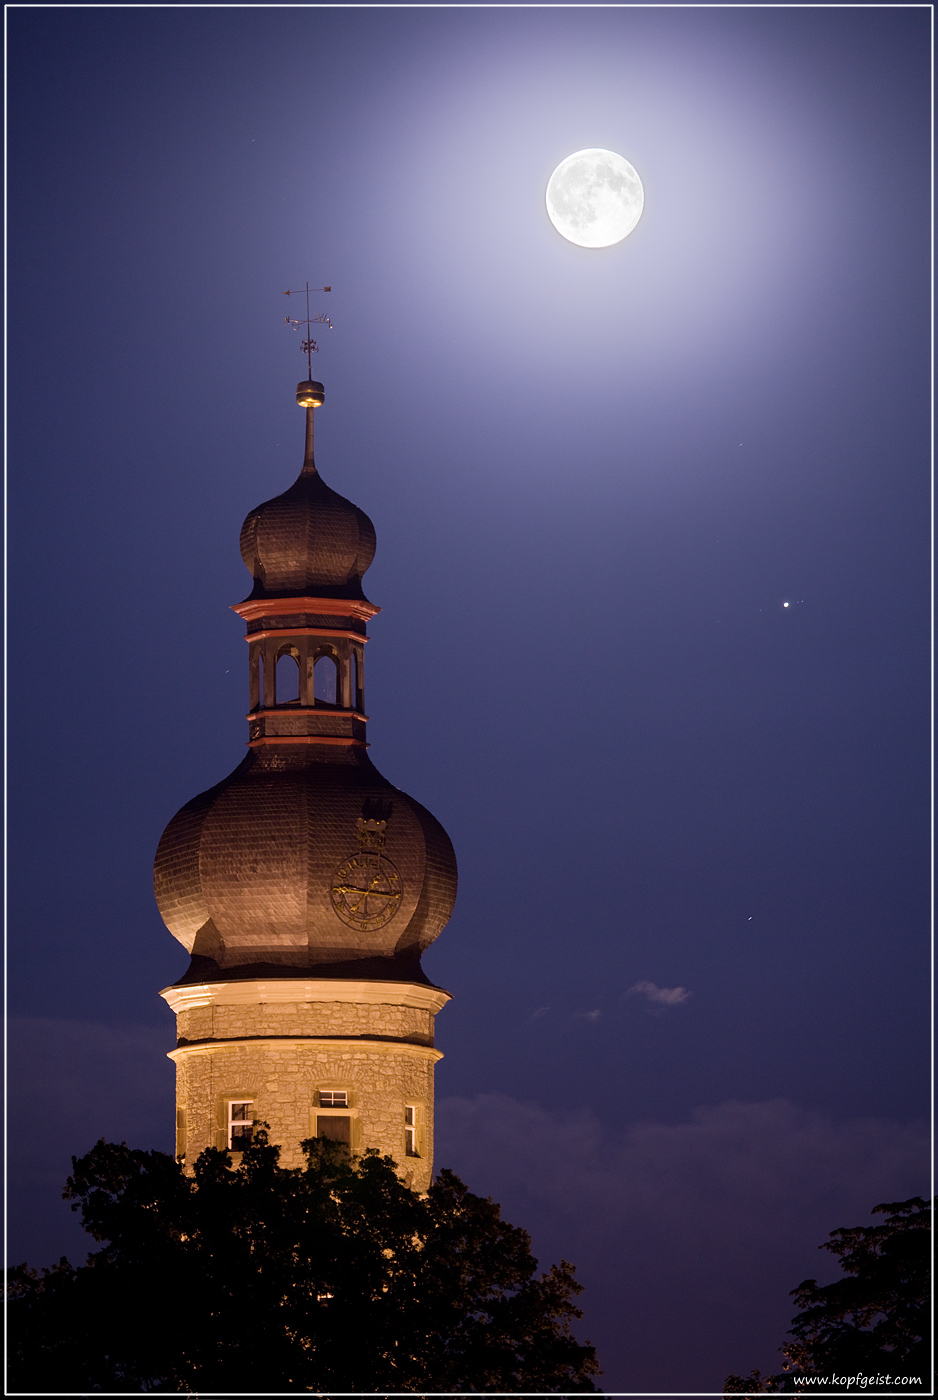
\includegraphics[width=\textwidth]{moonjupiter_hackmann.jpg}\EC
\column{0.6\textwidth}
\huge

\BC{\it ``And yet it moves."}\EC
\bigskip 
\large
\begin{flushright}--Galileo (attributed), on the Earth\end{flushright}
\end{columns}
}

\frame{\frametitle{\textbf{Announcements}}
\Large
\BI
\item This week's lab is Lab 4 
\item There may or may not be a prelab for next week; I'll let you know Thursday
\pause 

\BS

\item Papers are due Wednesday at 5PM:
\BI
\item Email a copy to \url{suast101projects@gmail.com}
\item Put a physical copy in your TA's mailbox
\item Check the lab schedule link on the website to look up your TA
\item This includes E. Nastas' former sections; your new TA is listed
\EI

\item Late paper submissions will lose 2 points per day 
\item If only your physical submission was late, talk to your TA
\EI
}

{
\setbeamercolor{background canvas}{bg=white}
\frame{\frametitle{\textbf{Exam grades}}
\BC
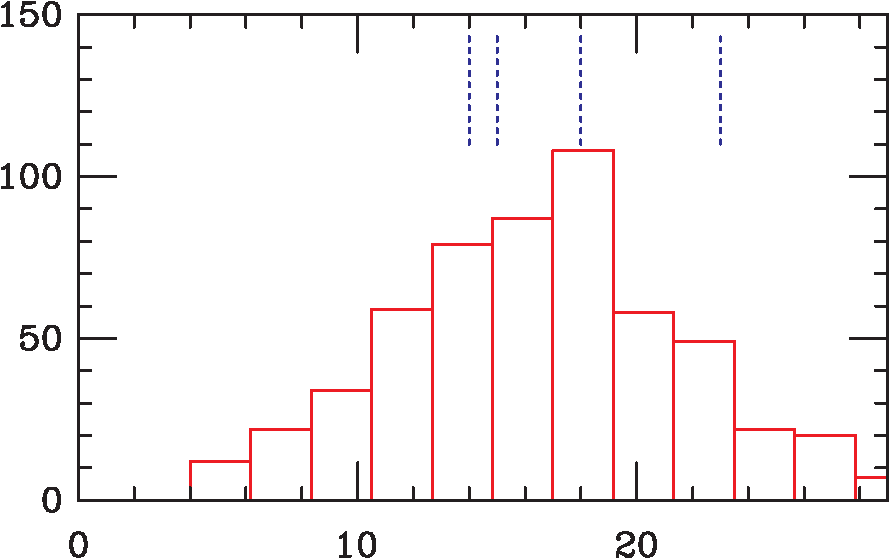
\includegraphics[width=0.6\textwidth]{exam-grade-histo-crop.pdf}

(Includes bonus questions on the exam; does not include other extra credit)

\EC
}
}

\frame{
	\large
	This exam was difficult. 
	
	\BS\BS
	
	Exam 1 is always the hardest exam in AST101, simply because this first unit involves so much spatial reasoning and geometry. This year's was particularly difficult.
	
	\BS
	
	For many of you this will have been the hardest exam you've taken in your life so far.\pause
	
	\BS
	
	If you did well, congratulations.
	
	\BS
	
	If you didn't do as well as you'd hoped, don't worry:
	
	\BI
	\item The other exams are somewhat easier
	\item We drop the lowest exam grade
	\item Many students' overall grades in AST101 are significantly higher than exam grades, because of labs, papers, and the final project
	\item This year we also have the in-class quizzes, which are sort of free points. (You can even use your notes for them!)
	\pause
	\item \bf If you do better on the questions on this material on the final than you did on Exam 1, you can raise your Exam 1 grade

	\EI
	
}

\frame{
	\large
	Some advice for preparing for the next exam:
	
	\BI
	\item Make sure you're staying current on the {\it Lecture Tutorials} work
	\item Factual recall isn't as important as being able to figure things out on the fly
	\item The next exam will involve a lot less geometry, but will involve reasoning with proportions
	
	\pause \bigskip\bigskip
	
	\item Make sure you're using the previous exam wisely:
	\BI
	\item Look for broad themes between the questions: how do different questions relate?
	\item It's not enough just to know the answers\pause
	\item It's {\color{Red}also} not enough to know how to figure out the answers\pause
	\item \bf Instead, for each question, ask: ``How would I know what to do here?''
	\EI
	\EI
}



\frame{\frametitle{\textbf{Last time}}

\Large\BC We left our story with two plausible models for the heavens: \EC

\begin{columns}
\column{0.5\textwidth}
\large
\BC The geocentric Ptolemaic model \EC


\column{0.5\textwidth}
\large
\BC The heliocentric Copernican model \EC
\end{columns}

\begin{columns}
\column{0.5\textwidth}
\normalsize
\BC 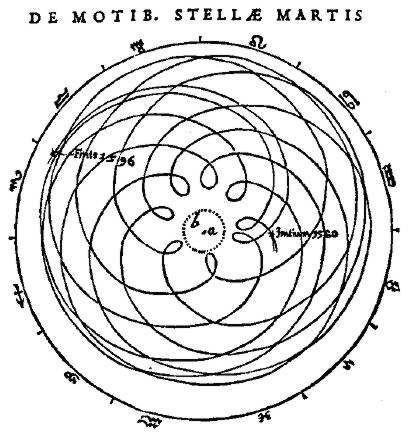
\includegraphics[width=0.4\textwidth]{epicycles.jpg}\EC
\BI
\item{The planets (and everything else) revolve around Earth}
\item{Inelegant system of ``epicycles'' needed to get planets right}
\item{Everything moved in circles (elegant per Greeks)}
\item{Earth and humanity at center (theologically not challenging)}
\item{\color{Red}Very accurate predictions}
\EI
\column{0.5\textwidth}
\normalsize
\BC 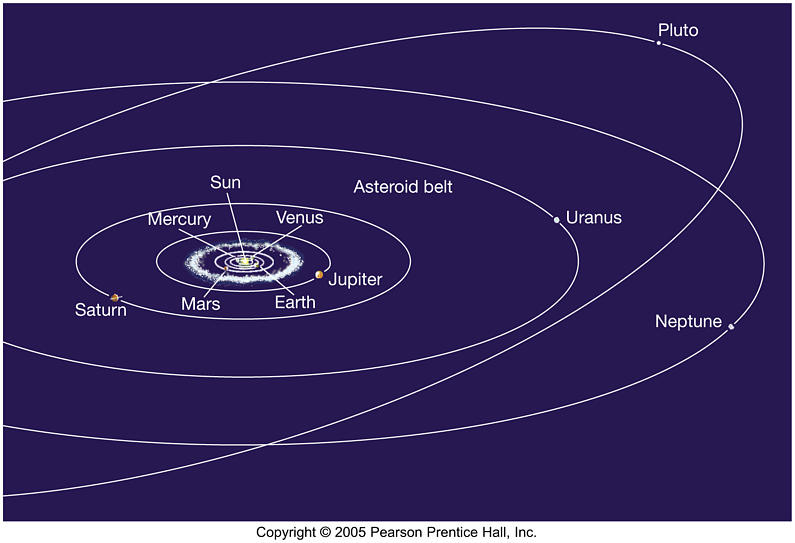
\includegraphics[width=0.46\textwidth]{ss-modern.jpg} \EC
\BI
\item{Earth is one of many planets, all orbiting the Sun}
\item{Apparent motion = motion of Earth + motion of planets}
\item{No (or very small) epicycles}
\item{\color{Red}Less accurate than Ptolemaic model}
\item{Matched Galileo's observations:}
\BI
\item{Moons of Jupiter}
\item{Phases of Venus}
\EI
\EI
\end{columns}
}




\frame{
\Large
The Copernican model had a lot of attractive features, but was still less accurate -- less good at actually telling you where the things in the sky would be!

\bigskip
\bigskip
\bigskip

Science doesn't attempt to explain the world ``only a little bit'' -- if Nature is based on underlying physical
laws, they should predict {\it \color{Red} everything!}

\bigskip

Is there a refinement of the Copernican model we can make?


\BI
\pause
\item{Different circular orbits?}
\pause
\item{Epicycles again?}
\pause
\item{Different shapes?}
\pause
\item{This is hard because now we have to think about both the Earth and the planets (see simulation)}
\pause
\item{What do we do?}
\EI
}

\frame{\frametitle{\textbf{What do we do when we don't know what to do?}}
\Large

Maybe our data are wrong...

\bigskip

The measurements of the sky that people had been using were ``good enough'' for navigation, but
they weren't ever intended for precision natural philosophy: determining the truth of things...

\bigskip

(In astronomy sometimes it is okay to round things off, and sometimes you need precise measurements to figure things out: 
you have to think carefully about this!)

\bigskip

\pause

Enter Tycho Brahe.

}

\frame{\frametitle{\textbf{Tycho Brahe}}

\begin{columns}

\column{0.5\textwidth}
\BC
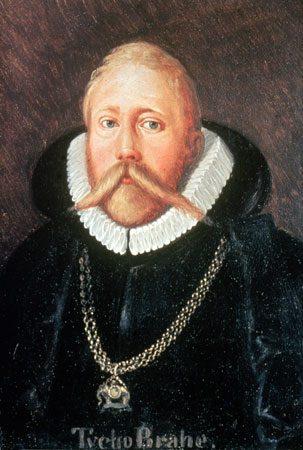
\includegraphics[width=0.8\textwidth]{tycho.jpg}
\EC

\column{0.5\textwidth}
\BI
\item{Danish nobleman and astronomer, 1546-1601}
\item{Built a fancy castle called Uraniborg to do research}
\item{Levied huge taxes on peasants to pay for it}
\pause
\item{Lost a big chunk of his nose in a duel and got a brass replacement made}
\pause
\item{Had better facial hair than any of us}

\EI

\end{columns}
}

\frame{\frametitle{\textbf{Tycho Brahe}}
	
	\begin{columns}
		
		\column{0.5\textwidth}
		\BC
		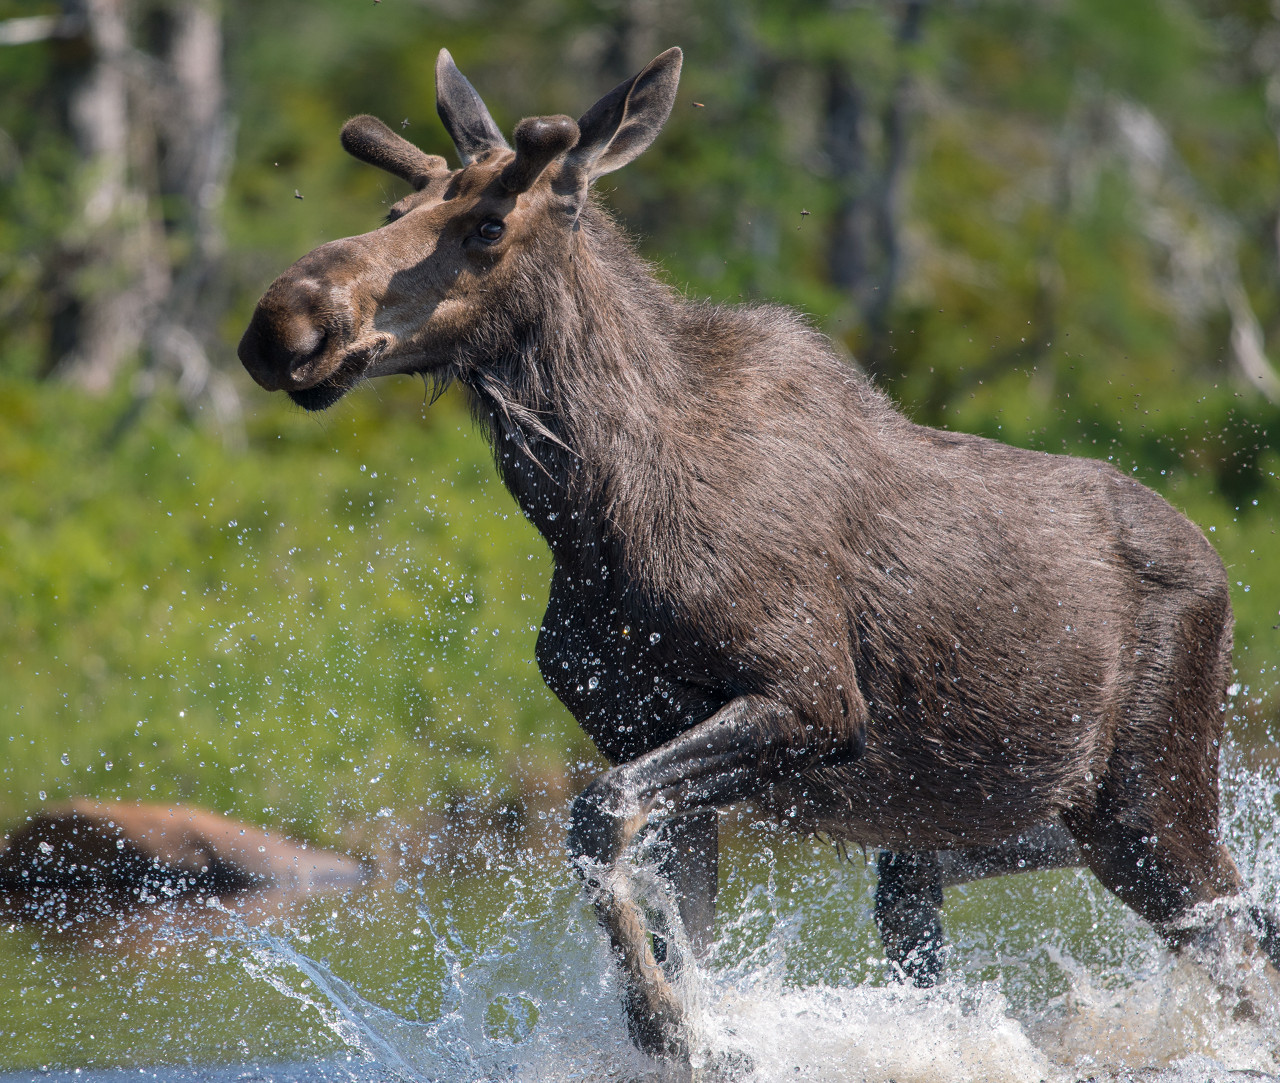
\includegraphics[width=\textwidth]{moose.jpg}
		\EC
		
		\column{0.5\textwidth}
		\BI
		\item{Danish nobleman and astronomer, 1546-1601}
		\item{Built a fancy castle called Uraniborg to do research}
		\item{Levied huge taxes on peasants to pay for it}
		\item{Lost a big chunk of his nose in a duel and got a brass replacement made}
		\item{Had better facial hair than any of us}
		\item{Had a pet moose}
		\EI
		
	\end{columns}
}

\frame{\frametitle{\textbf{Tycho Brahe}}
	
	\begin{columns}
		
		\column{0.5\textwidth}
		\BC
		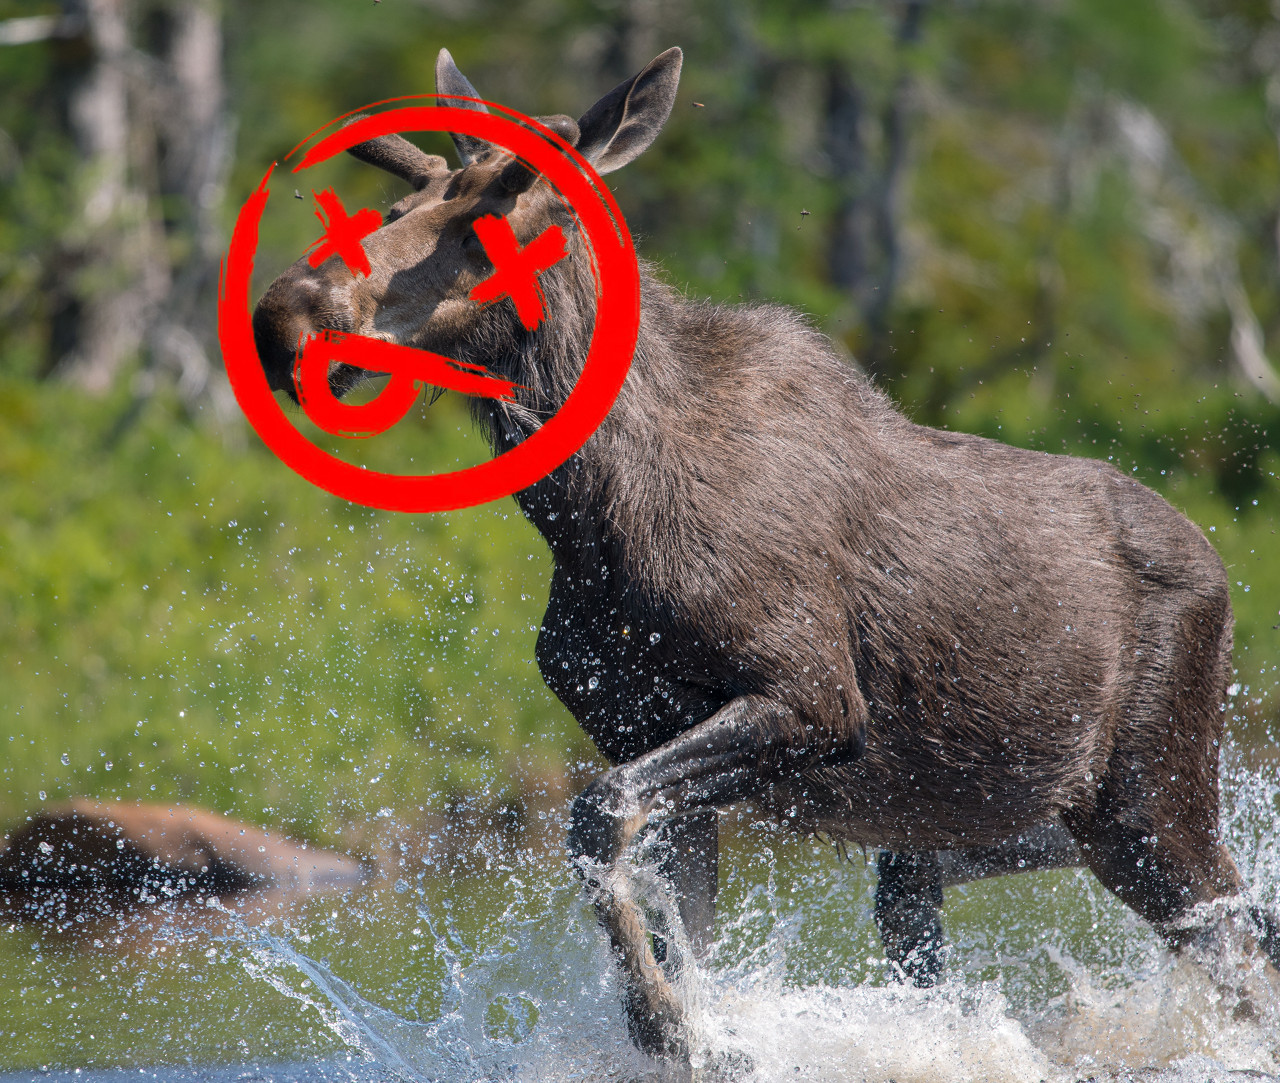
\includegraphics[width=\textwidth]{moose-dead.jpg}
		\EC
		
		\column{0.5\textwidth}
		\BI
		\item{Danish nobleman and astronomer, 1546-1601}
		\item{Built a fancy castle called Uraniborg to do research}
		\item{Levied huge taxes on peasants to pay for it}
		\item{Lost a big chunk of his nose in a duel and got a brass replacement made}
		\item{Had better facial hair than any of us}
		\item{Had a pet moose}
		\item{It drank too much beer and died}
		\item Was probably fun at parties (less so post-moose-death)
		\EI
		
	\end{columns}
}



\frame{\frametitle{\textbf{Tycho Brahe}}

\begin{columns}
\column{0.5\textwidth}
\BC
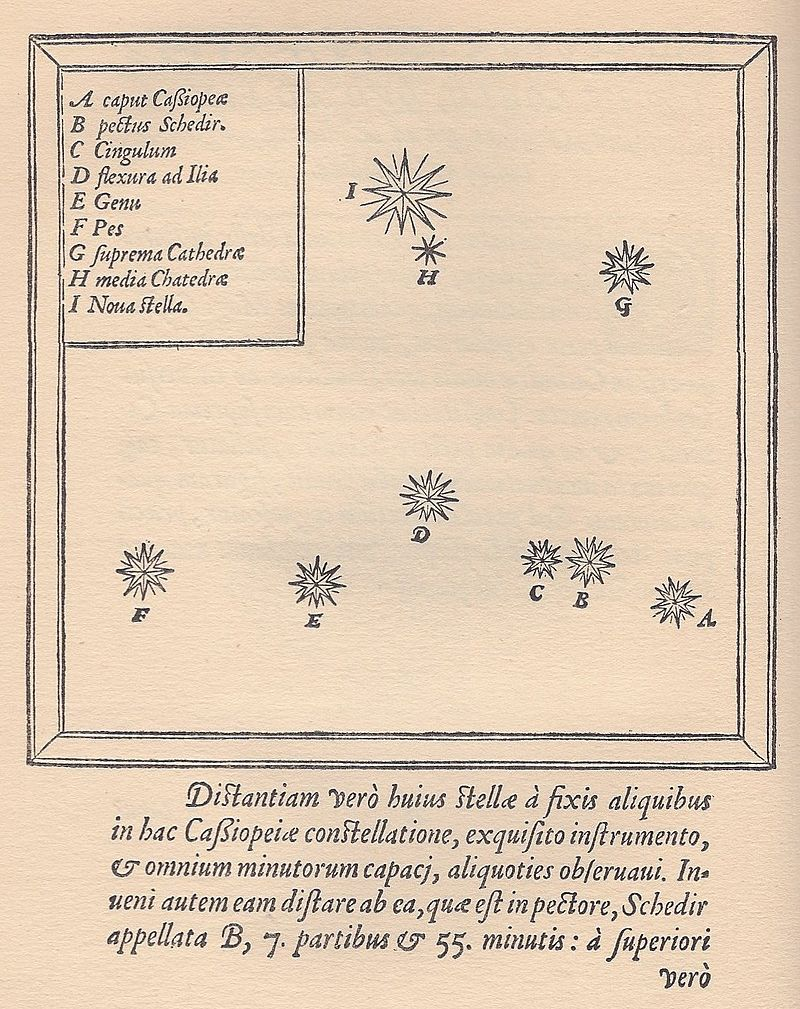
\includegraphics[width=0.8\textwidth]{tycho-supernova.jpg}
\EC
\column{0.5\textwidth}
\BI
\item{Danish nobleman and astronomer, 1546-1601}
\item{Observed a supernova in the constellation Cassiopeia}
\item{Old worldview: world beyond the Moon is eternal}
\item{... nope: no observed parallax in the supernova $\rightarrow$ it's very far away!}
\pause
\item{Didn't observe parallax in the distant stars}
\item{Two options:}
\BI
\item{The Earth doesn't move}
\item{The stars are very far away}
\EI
\item{He believed the former}
\item{Proposed another model for the Solar System}
\EI

\end{columns}
}


\frame{\frametitle{\textbf{Tycho Brahe}}

\begin{columns}
\column{0.5\textwidth}
\BC
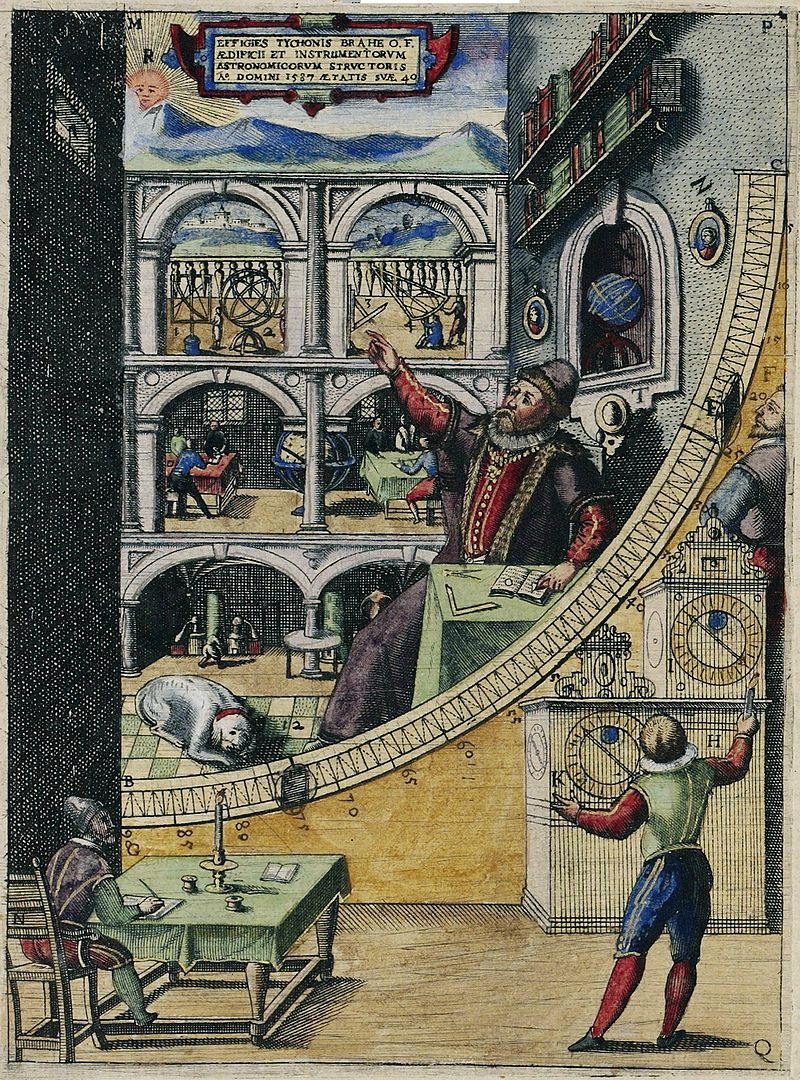
\includegraphics[width=0.8\textwidth]{uraniborg.jpg}
\EC
\column{0.5\textwidth}
\BI
\item{Danish nobleman and astronomer, 1546-1601}
\item{Best known for his precision measurements of the sky from Uraniborg}
\item{Made high precision observations of the motions of the planets and stars}
\item{Even had a crude correction for atmosphere bending light}
\item{Measurements accurate to a few minutes of arc (1/60'ths of a degree!)}
\item{Made these measurements with his assistant Sophie...}
\item{... and his later assistant Johannes Kepler, who didn't murder him}
\EI
\end{columns}
}


\frame{\frametitle{\textbf{Johannes Kepler}}
\BC
\Large
You've probably been wondering when we're going to stop this history of false starts and learn how things actually {\it do} work...

\bigskip
\pause

... here we go. Kepler, Tycho's assistant, finally got it right.

\bigskip

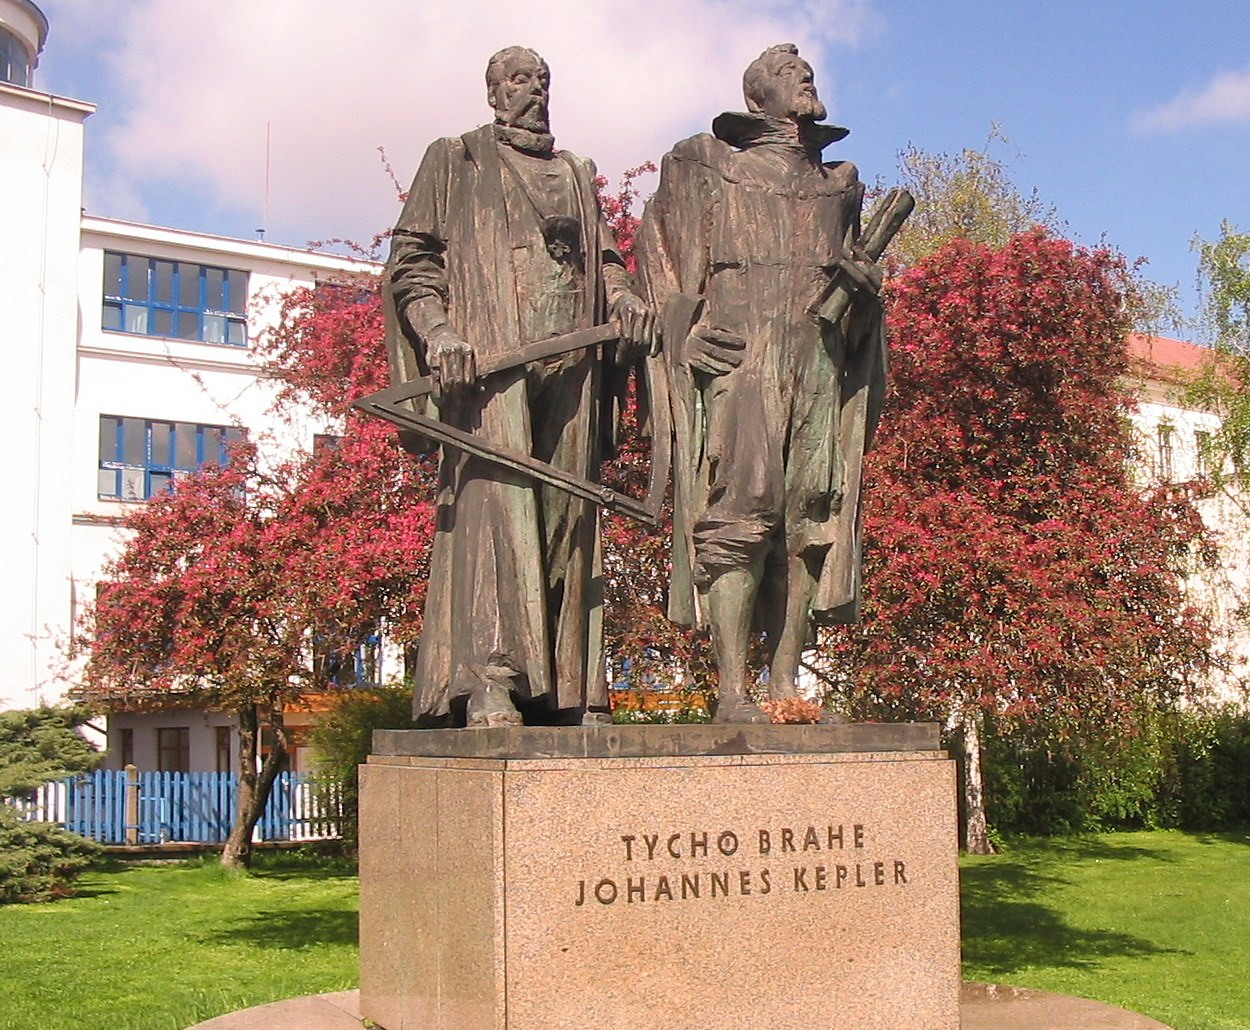
\includegraphics[width=0.5\textwidth]{tycho_kepler.jpg} \EC

}

\frame{
\Large
Kepler was a Copernican, and disagreed with his boss.

\bigskip

He tried to improve Copernicus' model, which used circular orbits, and mostly succeeded. But...

\BI
\item{Tycho's data were incredibly precise}
\item{No matter how he rearranged the circles, there was an error of at least 8/60 of a degree for Mars}
\item{Kepler worked at Uraniborg -- he knew how precise the data could be}
\EI

\pause

Do we:

\BI
\item{\color{A}A: Reject the belief that Nature must be elegant}
\item{\color{B}B: Reject the need for our model to match the data precisely}
\item{\color{C}C: Reject Tycho's data?}
\item{\color{D}D: Reexamine our ideas about what elegance looks like}
\EI 
}

\frame{
\Large
{``\it If I had believed that we could ignore that 8/60 of a degree, I would have patched up my hypothesis accordingly. But, since it was not 
permissible to ignore, those eight minutes pointed the road to a complete reformation in astronomy.''} --Kepler


\pause
\bigskip
\bigskip
\bigskip

{``\it There is a force in the Earth which causes the Moon to move.''} --Kepler, to Archduke Ferdinand

\bigskip
\bigskip
\bigskip
\pause
Kepler didn't only want to discover {\it how the planets moved}; he wanted to know {\it why}. He didn't figure it out, but he was on
the path that led to modern science.

\bigskip
\bigskip

Even if the {\it answer} doesn't have the perfect elegance of circles, modern science looks for its elegance in {\it laws}, not in 
all of their consequences! Kepler discovered the consequences; the laws weren't uncovered yet.
}


\frame{\frametitle{\textbf{Kepler's laws of planetary motion}}
\Large

\begin{enumerate}

\item The planets move in {\it ellipses}, with the Sun at one focus

\bigskip
\bigskip

\item The line joining the planet and the Sun sweeps out equal areas in equal times \\
Alternate formulation: Within its orbit, a planet's speed is inversely proportional to its distance from the Sun
\bigskip
\bigskip

\item The square of the orbital period of a planet is directly proportional to the cube of the semi-major axis of the ellipse.
\bigskip
\bigskip

\end{enumerate}


Let's talk about each of these in turn.
}

\frame{\frametitle{\textbf{Kepler's first law}}
\large
An ellipse is just a stretched circle. Mathematically: it's the curve around two points such that the {\it sum} of the distances to 
those points is a constant. A circle is just an ellipse with both foci at the same point.

\BC
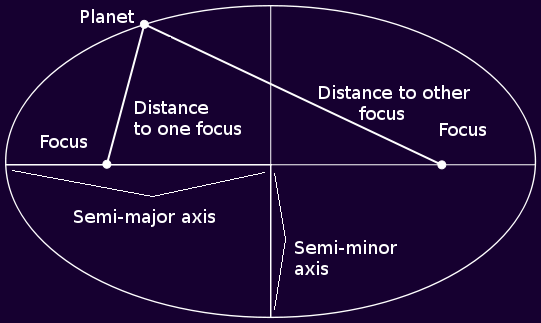
\includegraphics[width=0.6\textwidth]{ellipse.png}
\EC

Some terms:
\BI
\item{Focus: One of the two points}
\item{Semimajor axis: the largest distance from the center to the edge}
\item{Eccentricity: how stretched out an ellipse is}
\EI
}

\frame{\frametitle{\textbf{Some properties of ellipses}}
\large

\BC
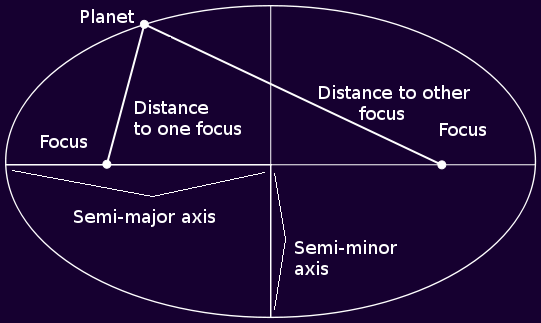
\includegraphics[width=0.6\textwidth]{ellipse.png}
\EC

\BI
\item{The two foci always lie along the major axis (``wide axis'')}
\item{The closer together the foci, the less eccentric}
\item{If both foci are exactly at the middle, you get a circle}
\item{Both foci lie inside the ellipse}
\EI
}




\frame{
\Large
Here's an orbit. Which is the correct position for the Sun?

\BC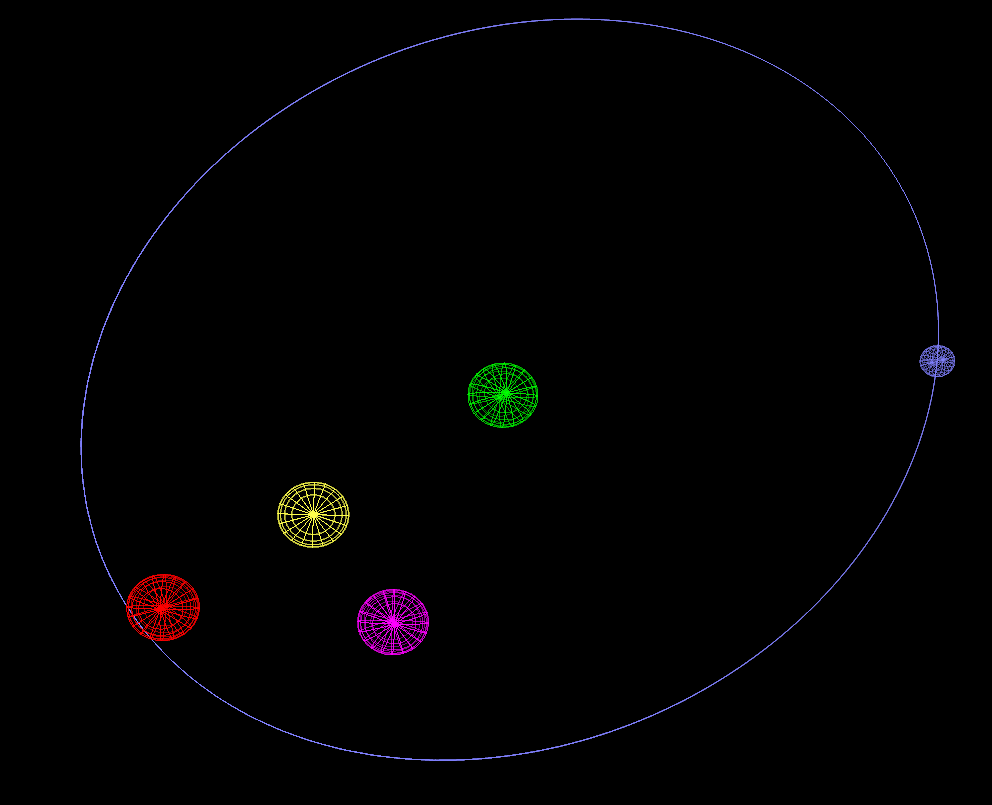
\includegraphics[width=0.5\textwidth]{ellipse-question1.png}\EC


\bigskip

\color{A}A: The red one\\
\color{B}B: The green one\\
\color{C}C: The yellow one\\
\color{D}D: The purple one\\
}

\frame{\frametitle{\textbf {What you need to know}}
	
	\Large
	
	\BI
	
	\item Planetary orbits are ellipses
	\item The {\it eccentricity} of an ellipse tells you how squashed it is
	\item An ellipse with zero eccentricity is just a circle
	
	\BS
	
	\item The Sun lies at a focus of the ellipse, which isn't at the center (unless it's a circle)
	\item The more eccentric the orbit, the further to one side the Sun is
	
	\EI
}


\frame{\frametitle{\textbf{Kepler's second law}}
\Large

In an eccentric orbit, a planet travels fastest when it's nearer the Sun.

\bigskip

\BC
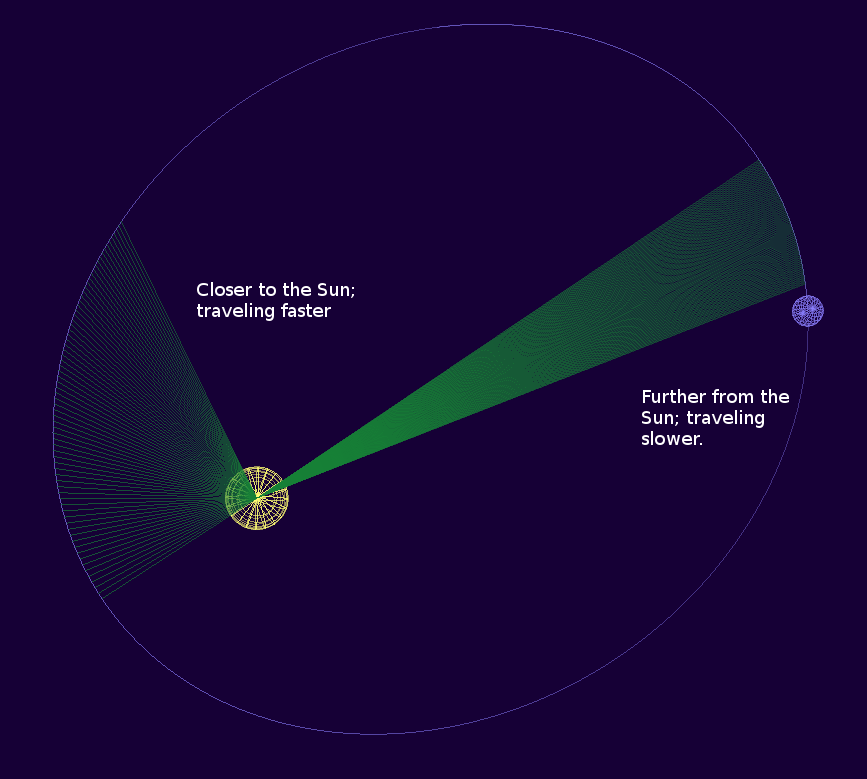
\includegraphics[width=0.5\textwidth]{second-law.png}
\EC

\pause

Let's watch this in an animation...

}

\frame{\frametitle{\textbf{Comets}}

\Large
Comets have highly eccentric orbits. Halley's Comet's furthest point from the Sun -- its {\it aphelion} -- is 35 AU away.
But its {\it perihelion} -- the nearest point to the Sun -- is 0.6 AU away.

\bigskip
\bigskip

Which statement is true?

\color{A}A: Halley's Comet spends most of its time far from the Sun, and only a little time near the Sun \\
\color{B}B: Halley's Comet moves slowly near perihelion, and quickly at aphelion  \\
\color{C}C: Halley's Comet moves quickly near perihelion, and slowly at aphelion \\
\color{D}D: Halley's Comet spends roughly equal amounts of time near the Sun, and far from it 

\bigskip
\bigskip
\bigskip
\pause
\BC
(Get creative with your folding...)
\EC

}


\frame{

\BC
\Huge
Complete {\it Lecture Tutorials} pp. 21-24.
\bigskip
\bigskip

\Large
We will do something else after this.
\EC
}

\frame{\frametitle{\textbf{Kepler's Third Law}}

\Large
Kepler's third law of orbital motion says that the square of a planet's {\it orbital period} is proportional
to the cube of its {\it semimajor axis}.

\bigskip
\bigskip
\bigskip

Simply put: if a planet is further from the Sun, it takes longer to go around.

\bigskip
\bigskip
\bigskip

If the distance is doubled, the time required {\it more than doubles}.

\bigskip
\bigskip
\bigskip

Let's watch this...

}

\frame{

\BC
\Huge
Complete {\it Lecture Tutorials} pp. 25-28.
\bigskip
\bigskip
\EC
}


\end{document}
